\documentclass[10pt]{article}
\usepackage{graphicx}
\usepackage{amssymb}
\usepackage[fleqn]{amsmath}
\usepackage{nccmath}
\usepackage{cases}
\usepackage{hyperref}
\usepackage{multicol}
\usepackage{tikz}
\usepackage{pgfplots}
\usepackage{enumitem}
\pgfplotsset{compat=1.18}
\usepackage{float}
\usepackage{pdfpages}

\title{\bf Math 116: Problem Set 2}
\date{1/21/2024}
\author{\bf Owen Jones}
\begin{document}
\maketitle
\begin{enumerate}[label=\arabic*.]
    \item $x_{n+3}=c_0x_n+c_1x_{n+1}+c_2x_{n+2}\\
    \Rightarrow \begin{bmatrix}
        0 & 0 & 1\\
        0 & 1 & 1\\
        1 & 1 & 1
    \end{bmatrix}\begin{bmatrix}
        c_0\\
        c_1\\
        c_2
    \end{bmatrix}=\begin{bmatrix}
        1\\
        1\\
        0
    \end{bmatrix}\\
    \Rightarrow (c_0,c_1,c_2)=(1,0,1)\\
    \Rightarrow x_{n+3}=x_n+x_{n+2}\\
    \Rightarrow 1001$ are the next $4$ elements of the sequence.
    \item $\det(M_3)=\det\begin{bmatrix}
        1 & 0 & 1\\
        0 & 1 & 0\\
        1 & 0 & 1
    \end{bmatrix}=1+0-1=0\mod 2\\
    \Rightarrow \begin{bmatrix}
        1 & 0\\
        0 & 1
    \end{bmatrix}\begin{bmatrix}
        c_0\\
        c_1
    \end{bmatrix}=\begin{bmatrix}
        1\\
        0
    \end{bmatrix}\\
    \Rightarrow (c_0,c_1)=(1,0)\\
    \Rightarrow x_{n+2}=x_n$
    \item \begin{enumerate}
        \item If Eve observes the ciphertext repeats with a period of $6$, she can deduce that the plaintext is one repeated letter and the key is length $6$.
        Eve knows every $n-th$ character will be shifted by the same amount, and she notices every $6th$ letter is the same.
        If the key is of length $6$, then every $6th$ letter is the same letter.
        Since each of the congruence classes $\mod6$ are shifted by different amounts, a good guess is to assume that every character is the same letter.
        \item Using the property that no $6$ letter word is a shift of another word, the fastest way to determine the key is by brute force. 
        Shift the first $6$ characters of the ciphertext by $1\mod 26$ until an English word is obtained.
        \item \# of matches = $\begin{cases}
            \text{length of ciphertext}-n & \text{ for }n\equiv0\mod6\\
            0 & \text{ for }n\not\equiv0\mod6
        \end{cases}$\\
        where n is the number of displacements.
    \end{enumerate}
    \item The message is EVEISEAVESDROPPINGONUS
    \item The key is JACK and the message is WEUSEWORDSLIKEHONORCODELOYALTYWEUSETHESEWORDSASTHEBACKBONE
    OFALIFESPENTDEFENDINGSOMETHINGYOUUSETHEMASAPUNCHLINEIHAVENEITHERTHETIMENORTHEINCLINATIONTOEXPLAIN
    MYSELFTOAMANWHORISESANDSLEEPSUNDERTHEBLANKETOFTHEVERYFREEDOMTHATIPROVIDEANDTHENQUESTIONSTHEMANNER
    INWHICHIPROVIDEIT
    \item The key is WATSON and the message is 'HOLMESHADBEENSEATEDFORSOMEHOURSINSILENCEWITHHISLONG
    THINBACKCURVEDOVERACHEMICALVESSELINWHICHHEWASBREWINGAPARTICULARLYMALODOROUSPRODUCTHISHEADWASSUNK
    UPONHISBREASTANDHELOOKEDFROMMYPOINTOFVIEWLIKEASTRANGELANKBIRDWITHDULLGREYPLUMAGEANDABLACKTOPKNOT
    SOWATSONSAIDHESUDDENLYYOUDONOTPROPOSETOINVESTINSOUTHAFRICANSECURITIES'
\end{enumerate}
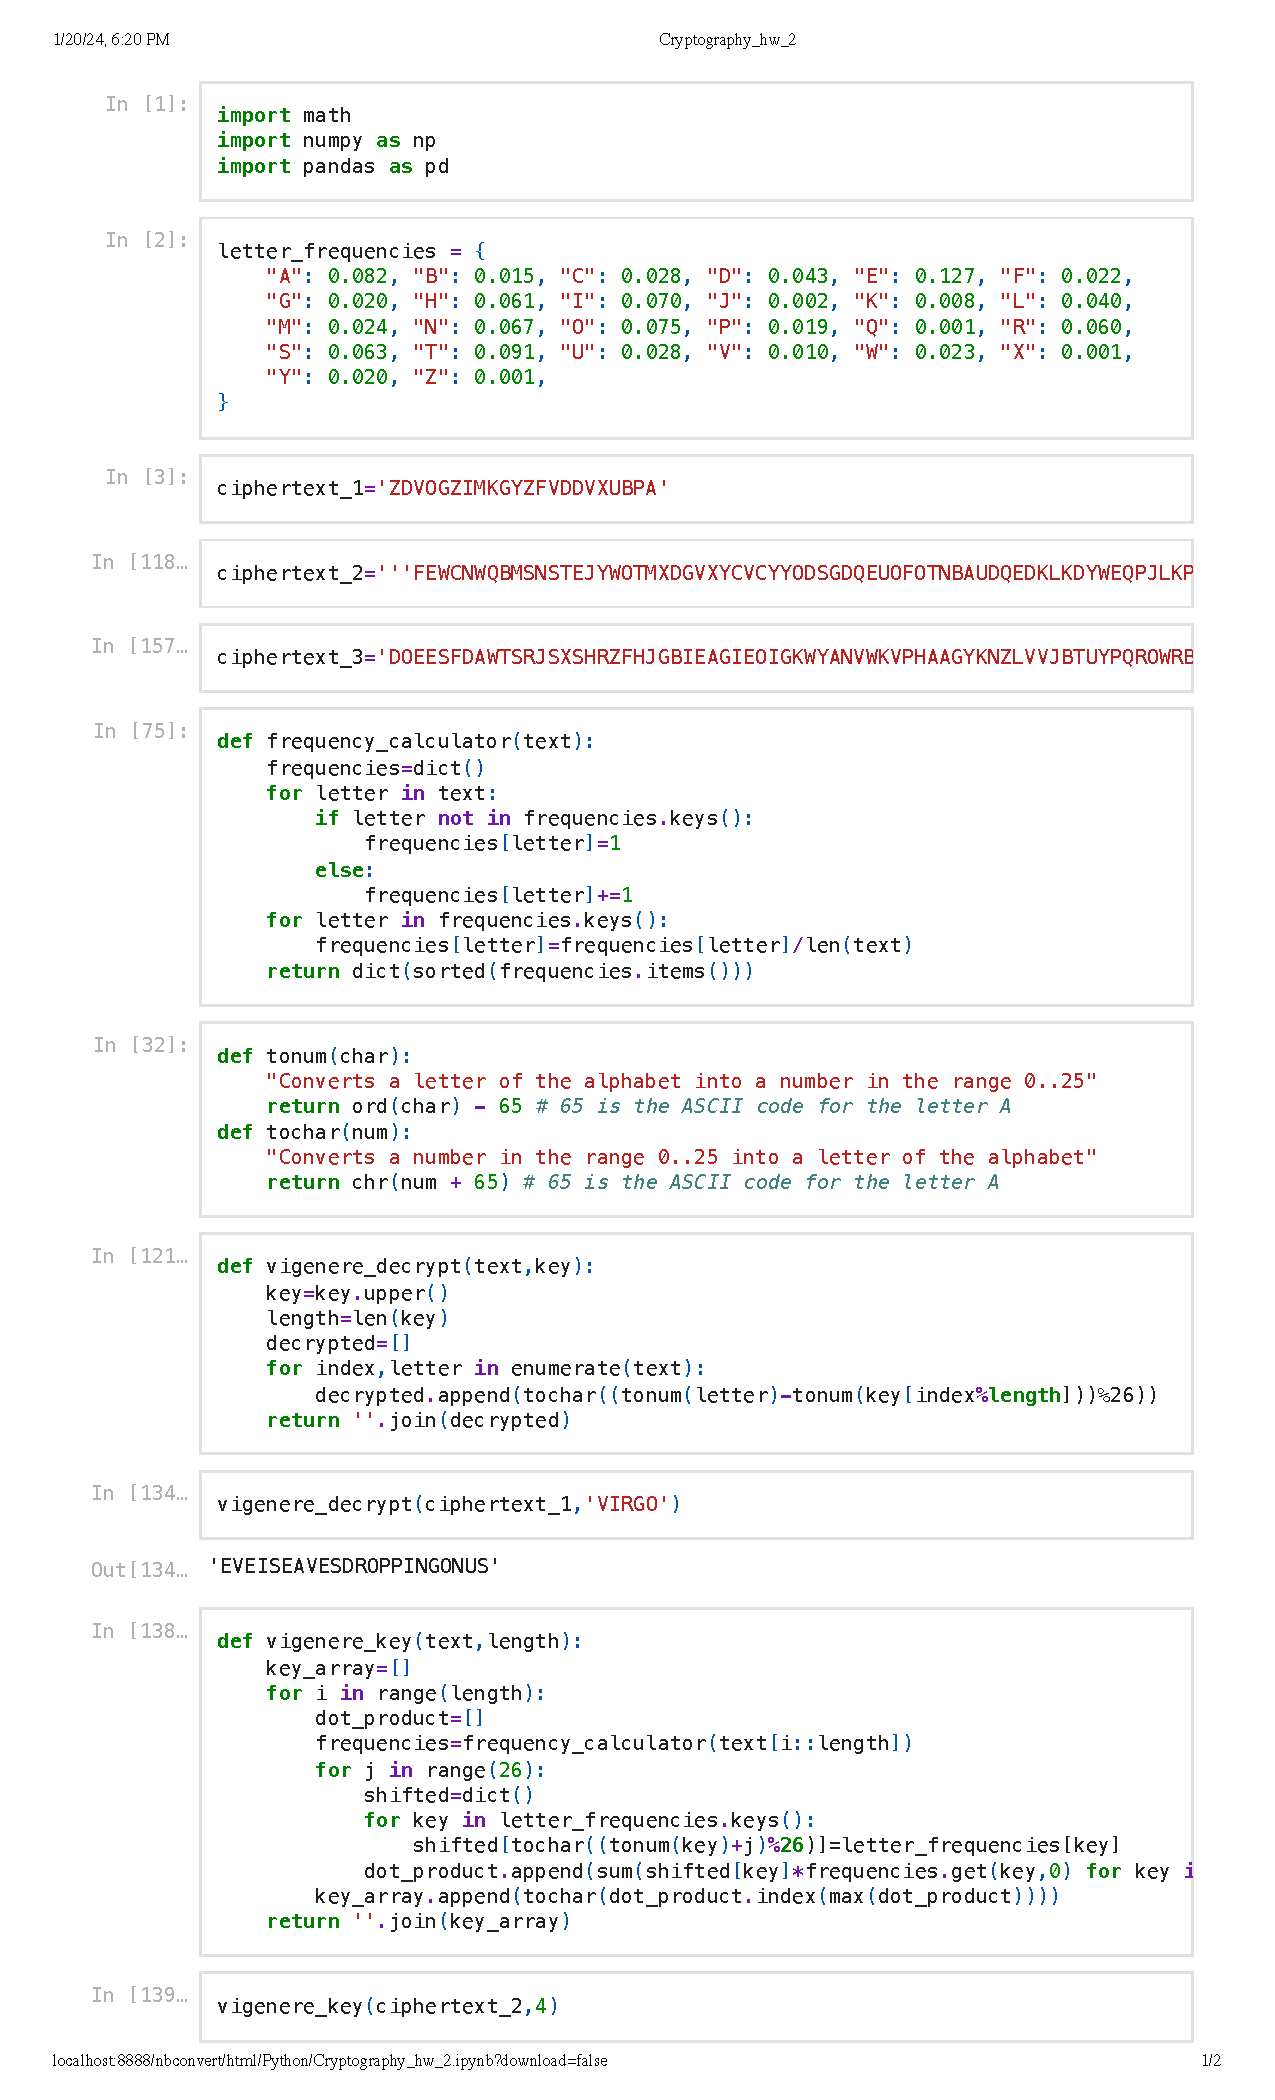
\includepdf[pages=-]{Cryptography_hw_2.pdf}
\end{document}